\documentclass[12pt]{article}
\usepackage[margin=1in]{geometry}
\usepackage{amsmath}
\usepackage{graphicx}
\usepackage[utf8]{inputenc}
\author{Henry Pick \small hpick@hmc.edu \\
\large Noah Nevens \small nnevens@hmc.edu \\
\large Prakod Ngamlamai \small pngamlamai@hmc.edu}
\title{HMC Room Draw Optimization}
\DeclareMathOperator*{\maxi}{max}
\begin{document}
    \maketitle
    \section*{Scratch Works}
    \begin{itemize}
        \item We have the first objective function: $\text{max} \sum_{(i,j) \in G_k \times R_k}  w_{ij}x_{ij}$ where $w_{ij}$ is the preference of group $i$ for room $j$. This would be the naive linear program that maximize the sum of the utility in a selection. 
        \item However, if we wish to maximize the minimum utility, then we consider another objective function \begin{align*}
            &\text{max  } m \\
            &s.t. &m &\leq w_{ij} + M*(1-x_{ij}) \\
            & &\sum_{i \in \text{Groups}}x_{ij} &\leq 1 \\
            & &\sum_{j \in \text{Rooms}}x_{ij} &= 1 \\
        \end{align*}
    \end{itemize}
    \section*{Frontend}
    Our project is supposed to be ``implementable'', which led us to focus on developing a frontend for collecting room preference data. In order to programmatically construct the models that will run our optimization, we need relational data. Thus, the frontend must be a little more complex than a simple google form. The general process that we have in mind is as follows:
    \begin{enumerate}
        \item A group of people submit a form together saying that they want to be roommates/suitemates
        \item In this form, they will provide a list of rooms or sections of dorms that they would prefer to be placed in. The preferences on these lists can be set relative to one another. There is a cumulative preference total that each form cannot exceed. For example, a group can rank a set of rooms with preferences $(1, 2, 3)$ or $(1.5, 1.5, 3)$ depending on whether they are indifferent about being placed in the first or second room in that list.
        \item The backend will receive the forms, validate their data, and push it to the database as relational data.
        \item Once the preference submissions have completed, a routine on the backend will run the optimization
    \end{enumerate}
    The infrastructure for this will thus be fairly simple: a web server with a relational database and HTML forms:
    \begin{center}
        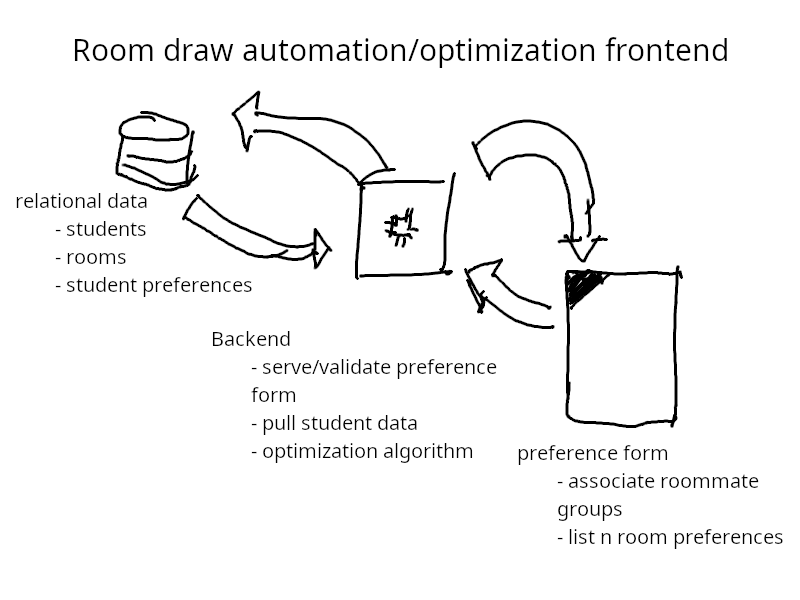
\includegraphics[width=0.9\linewidth]{frontend.png}
    \end{center}
    
\end{document}